%% GENERATED by tools/from_docs.py from stepss-docs. Do not edit by hand:
%% edit the page named below in stepss-docs and regenerate.
%% source: stepss-docs/src/content/docs/models/injectors/loads.md

\chapter{Load and equivalent models}\label{doc:model-inj-loads}

Injector models for loads (exponential, restorative, constant power, variable frequency drive) and for a Th\'evenin equivalent of an external system.

The \texttt{INJEC} record these models are entered with, and the rules on model names, are on the Injector Models page.

\section{\texorpdfstring{LOAD (\texttt{inj\_load}): Exponential Recovery Load}{LOAD (inj\_load): Exponential Recovery Load}}\label{model-inj-loads:load-inj_load-exponential-recovery-load}

\subsection{Description}\label{model-inj-loads:description}

The exponential recovery load model captures the transient and steady-state voltage and frequency dependency of aggregated loads. Immediately after a voltage disturbance, the load behaves according to a transient voltage exponent; it then recovers exponentially to a steady-state behaviour described by a different exponent. The model supports separate active (\(P\)) and reactive (\(Q\)) power recovery dynamics, each with individual minimum/maximum limiters on the recovery variable.

\begin{figure}[htbp]
\centering
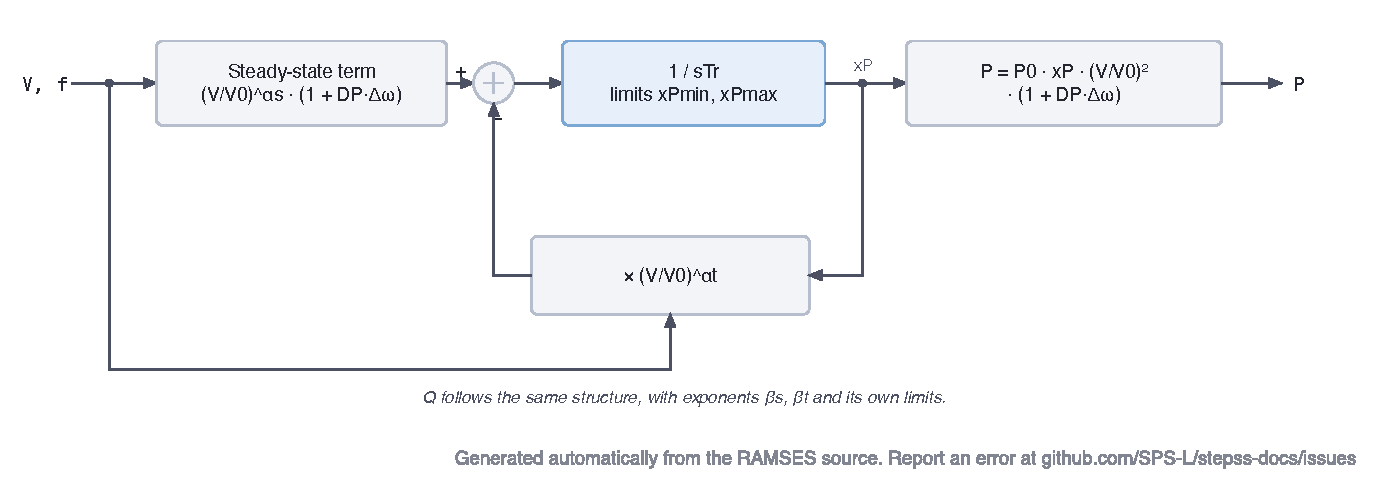
\includegraphics[width=0.98\linewidth]{figures/inj-load-light}
\caption{Exponential recovery load block diagram.}
\end{figure}

\subsection{Scientific Description}\label{model-inj-loads:scientific-description}

The model is parameterized in terms of initial active and reactive conductance/susceptance, \(G_0 = P_0/V_0^2\) and \(B_0 = -Q_0/V_0^2\). Two recovery state variables \(x_P\) and \(x_Q\) evolve according to:

\[\dot{x}_P = \frac{1}{T_r}\left[\left(\frac{V}{V_0}\right)^{\alpha_s} \left(1 + D_P\,\Delta\omega\right) - x_P \left(\frac{V}{V_0}\right)^{\alpha_t}\right]\]

\[\dot{x}_Q = \frac{1}{T_r}\left[\left(\frac{V}{V_0}\right)^{\beta_s} \left(1 + D_Q\,\Delta\omega\right) - x_Q \left(\frac{V}{V_0}\right)^{\beta_t}\right]\]

where \(\Delta\omega = \omega_{\mathrm{COI}} - 1\) is the per-unit speed deviation, \(V\) is the bus voltage magnitude, \(V_0\) is the initial voltage, \(\alpha_t, \beta_t\) are transient exponents, \(\alpha_s, \beta_s\) are steady-state exponents, and \(T_r\) is the load recovery time constant. The injected currents are then:

\[i_x = G_0\, x_P\, v_x\left(1 + D_P\,\Delta\omega\right) - B_0\, x_Q\, v_y\left(1 + D_Q\,\Delta\omega\right)\]

\[i_y = G_0\, x_P\, v_y\left(1 + D_P\,\Delta\omega\right) + B_0\, x_Q\, v_x\left(1 + D_Q\,\Delta\omega\right)\]

When the recovery variable hits its limit (due to e.g.~Stalling or complete voltage collapse), the limit is held until the direction of the derivative reverses.

\subsection{Parameters}\label{model-inj-loads:parameters}

\begin{small}\begin{longtable}[]{@{}
  >{\raggedright\arraybackslash}p{(\linewidth - 8\tabcolsep) * \real{0.1047}}
  >{\raggedright\arraybackslash}p{(\linewidth - 8\tabcolsep) * \real{0.1832}}
  >{\raggedright\arraybackslash}p{(\linewidth - 8\tabcolsep) * \real{0.5961}}
  >{\raggedright\arraybackslash}p{(\linewidth - 8\tabcolsep) * \real{0.1160}}
@{}}
\toprule\noalign{}
\begin{minipage}[b]{\linewidth}\raggedright
\#
\end{minipage} & \begin{minipage}[b]{\linewidth}\raggedright
Name
\end{minipage} & \begin{minipage}[b]{\linewidth}\raggedright
Description
\end{minipage} & \begin{minipage}[b]{\linewidth}\raggedright
Unit
\end{minipage} \\
\midrule\noalign{}
\endhead
\bottomrule\noalign{}
\endlastfoot
1 & \texttt{DP} & Frequency sensitivity of active power & pu/pu \\
2 & \texttt{A1} & Proportion of type-1 component in \(P\) & \\
3 & \texttt{alpha1} & Transient voltage exponent for \(P\) (type 1) & \\
4 & \texttt{A2} & Proportion of type-2 component in \(P\) & \\
5 & \texttt{alpha2} & Transient voltage exponent for \(P\) (type 2) & \\
6 & \texttt{alpha3} & Transient voltage exponent for \(P\) (type 3, proportion \(= 1-A_1-A_2\)) & \\
7 & \texttt{DQ} & Frequency sensitivity of reactive power & pu/pu \\
8 & \texttt{B1} & Proportion of type-1 component in \(Q\) & \\
9 & \texttt{beta1} & Transient voltage exponent for \(Q\) (type 1) & \\
10 & \texttt{B2} & Proportion of type-2 component in \(Q\) & \\
11 & \texttt{beta2} & Transient voltage exponent for \(Q\) (type 2) & \\
12 & \texttt{beta3} & Transient voltage exponent for \(Q\) (type 3) & \\
\end{longtable}\end{small}

Internal computed parameters include the steady-state exponents for each component (derived from the transient exponents), initial conductance \(G_0\), susceptance \(B_0\), and initial voltage \(V_0\).

\subsection{State Variables}\label{model-inj-loads:state-variables}

\begin{small}\begin{longtable}[]{@{}ll@{}}
\toprule\noalign{}
Variable & Description \\
\midrule\noalign{}
\endhead
\bottomrule\noalign{}
\endlastfoot
\texttt{iy} & \(y\)-component of injected current (pu on system base) \\
\texttt{ix} & \(x\)-component of injected current (pu on system base) \\
\texttt{xp} & Active power recovery variable (dimensionless) \\
\texttt{xq} & Reactive power recovery variable (dimensionless) \\
\end{longtable}\end{small}

\textbf{Observables:} \texttt{P}, \texttt{Q}, \texttt{xp}, \texttt{xq}

\subsection{Usage Example}\label{model-inj-loads:usage-example}

\begin{Verbatim}
INJEC  LOAD  LOAD1  BUS1
      # FP FQ P Q: share of the power-flow injection (FP, FQ) or initial power (P in MW, Q in Mvar)
      1.  1.  0.  0.
      # DP: Frequency sensitivity of active power (pu/pu)
      1.5
      # A1: Proportion of type-1 component in P
      0.3
      # alpha1: Voltage exponent of the A1 term of P
      1.0
      # A2: Proportion of type-2 component in P
      0.2
      # alpha2: Voltage exponent of the A2 term of P
      2.0
      # alpha3: Voltage exponent of the remaining (1-A1-A2) term of P
      0.5
      # DQ: Frequency sensitivity of reactive power (pu/pu)
      1.8
      # B1: Proportion of type-1 component in Q
      0.4
      # beta1: Voltage exponent of the B1 term of Q
      2.5
      # B2: Proportion of type-2 component in Q
      0.1
      # beta2: Voltage exponent of the B2 term of Q
      3.0
      # beta3: Voltage exponent of the remaining (1-B1-B2) term of Q
      2.0
;
\end{Verbatim}

\emph{Parameters: \texttt{DP\ A1\ alpha1\ A2\ alpha2\ alpha3\ DQ\ B1\ beta1\ B2\ beta2\ beta3}}

\begin{center}\rule{0.5\linewidth}{0.5pt}\end{center}

\section{\texorpdfstring{vfd\_load (\texttt{inj\_vfd\_load}): Variable Frequency Drive Load}{vfd\_load (inj\_vfd\_load): Variable Frequency Drive Load}}\label{model-inj-loads:vfd_load-inj_vfd_load-variable-frequency-drive-load}

\subsection{Description}\label{model-inj-loads:description-1}

The VFD load model represents aggregate industrial loads driven by variable-frequency drives, where the power consumption exhibits a composite voltage-dependent characteristic with multiple exponential components and frequency sensitivity. It also includes low-voltage protection: below a configurable threshold \(V_{\min}\), the load switches to a constant-admittance representation, preventing numerical difficulties during deep voltage sags.

\begin{figure}[htbp]
\centering
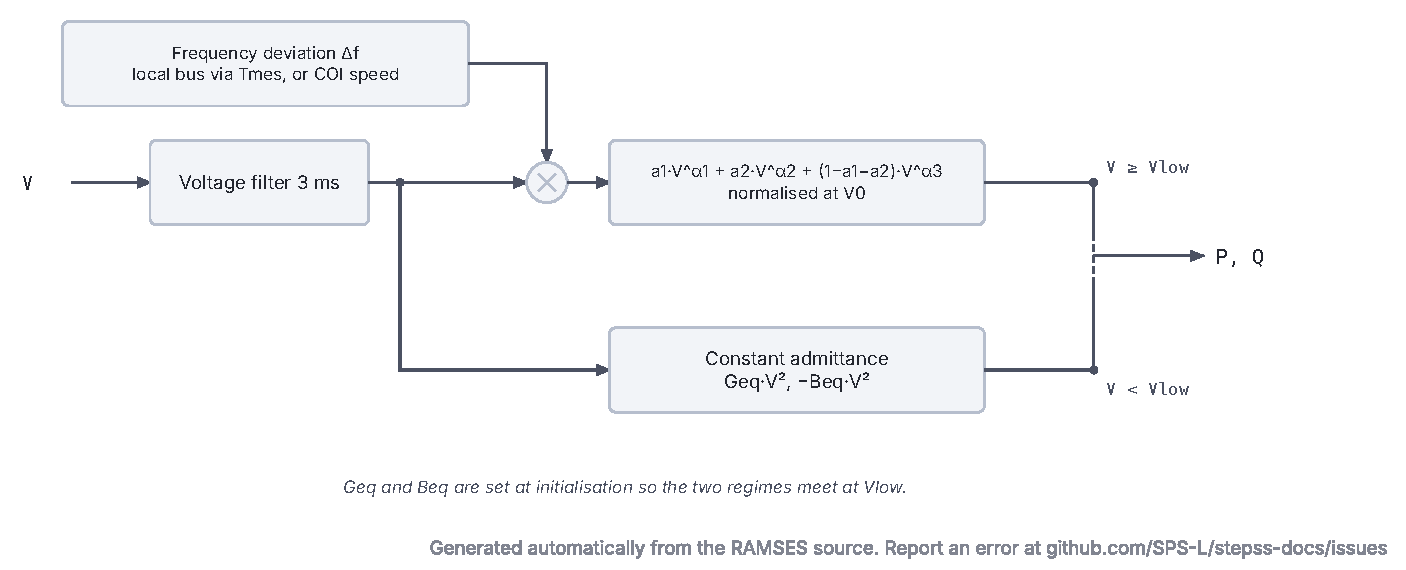
\includegraphics[width=0.98\linewidth]{figures/inj-vfd-load-light}
\caption{Variable frequency drive load block diagram.}
\end{figure}

\subsection{Scientific Description}\label{model-inj-loads:scientific-description-1}

The active and reactive powers depend on bus voltage \(V\) and frequency deviation \(\Delta f = f/f_0 - 1\):

\[P = \left(1 + D_P\,\Delta f\right) P_0 \cdot \frac{a_1 V^{\alpha_1} + a_2 V^{\alpha_2} + (1-a_1-a_2)\, V^{\alpha_3}}{a_1 V_0^{\alpha_1} + a_2 V_0^{\alpha_2} + (1-a_1-a_2)\, V_0^{\alpha_3}}\]

\[Q = \left(1 + D_Q\,\Delta f\right) Q_0 \cdot \frac{b_1 V^{\beta_1} + b_2 V^{\beta_2} + (1-b_1-b_2)\, V^{\beta_3}}{b_1 V_0^{\beta_1} + b_2 V_0^{\beta_2} + (1-b_1-b_2)\, V_0^{\beta_3}}\]

Below \(V_{\min}\), an equivalent constant admittance is used:

\[P_{\mathrm{low}} = G_{\mathrm{eq}}\, V^2, \qquad Q_{\mathrm{low}} = -B_{\mathrm{eq}}\, V^2\]

where \(G_{\mathrm{eq}}\) and \(B_{\mathrm{eq}}\) are computed at initialization to ensure continuity at \(V = V_{\min}\). The switch between the two regimes is governed by a piecewise-linear function of \(V\):

\[u = \begin{cases} 0 & V < V_{\min} \\ 1 & V \geq V_{\min} \end{cases}\]

A small voltage filter (time constant 0.003 s) smooths the transition. The frequency deviation can optionally be computed from the local bus frequency (measured via an \texttt{f\_inj} block with time constant \(T_{\mathrm{mes}}\)) or from the system centre-of-inertia speed.

The initial voltage \(V_0\) can differ from the transmission bus voltage if a distribution transformer ratio is implied (set \(V_{\mathrm{init}} \ne 0\) to specify the distribution-side voltage; otherwise the transmission voltage is used directly).

\subsection{Parameters}\label{model-inj-loads:parameters-1}

\begin{small}\begin{longtable}[]{@{}
  >{\raggedright\arraybackslash}p{(\linewidth - 8\tabcolsep) * \real{0.1092}}
  >{\raggedright\arraybackslash}p{(\linewidth - 8\tabcolsep) * \real{0.1851}}
  >{\raggedright\arraybackslash}p{(\linewidth - 8\tabcolsep) * \real{0.5926}}
  >{\raggedright\arraybackslash}p{(\linewidth - 8\tabcolsep) * \real{0.1130}}
@{}}
\toprule\noalign{}
\begin{minipage}[b]{\linewidth}\raggedright
\#
\end{minipage} & \begin{minipage}[b]{\linewidth}\raggedright
Name
\end{minipage} & \begin{minipage}[b]{\linewidth}\raggedright
Description
\end{minipage} & \begin{minipage}[b]{\linewidth}\raggedright
Unit
\end{minipage} \\
\midrule\noalign{}
\endhead
\bottomrule\noalign{}
\endlastfoot
1 & \texttt{Dp} & Frequency sensitivity of active power & pu/pu \\
2 & \texttt{a1} & Fraction of type-1 component in \(P\) & \\
3 & \texttt{alpha1} & Voltage exponent of type-1 \(P\) component & \\
4 & \texttt{a2} & Fraction of type-2 component in \(P\) & \\
5 & \texttt{alpha2} & Voltage exponent of type-2 \(P\) component & \\
6 & \texttt{alpha3} & Voltage exponent of type-3 \(P\) component (fraction \(= 1-a_1-a_2\)) & \\
7 & \texttt{Dq} & Frequency sensitivity of reactive power & pu/pu \\
8 & \texttt{b1} & Fraction of type-1 component in \(Q\) & \\
9 & \texttt{beta1} & Voltage exponent of type-1 \(Q\) component & \\
10 & \texttt{b2} & Fraction of type-2 component in \(Q\) & \\
11 & \texttt{beta2} & Voltage exponent of type-2 \(Q\) component & \\
12 & \texttt{beta3} & Voltage exponent of type-3 \(Q\) component & \\
13 & \texttt{Vinit} & Initial distribution-bus voltage (0 = use transmission voltage) & pu \\
14 & \texttt{Vlow} & Voltage threshold for constant-admittance regime (recommended 0.5--0.7) & pu \\
15 & \texttt{foption} & 1 = use local bus frequency; 0 = use COI speed & flag \\
16 & \texttt{Tmes} & Frequency measurement time constant & s \\
\end{longtable}\end{small}

\subsection{State Variables}\label{model-inj-loads:state-variables-1}

\begin{small}\begin{longtable}[]{@{}ll@{}}
\toprule\noalign{}
Variable & Description \\
\midrule\noalign{}
\endhead
\bottomrule\noalign{}
\endlastfoot
\texttt{Vreal} & Voltage at equivalent distribution bus \\
\texttt{V} & Filtered distribution-bus voltage (3 ms filter) \\
\texttt{P} & Active power consumed \\
\texttt{Q} & Reactive power consumed \\
\texttt{fbus} & Local bus frequency (used if \texttt{foption=1}) \\
\texttt{df} & Frequency deviation \(\Delta f\) \\
\texttt{u} & Regime switch (1 = above \(V_{\min}\), 0 = constant admittance) \\
\end{longtable}\end{small}

\textbf{Observables:} \texttt{P}, \texttt{Q}, \texttt{df}, \texttt{u}

\subsection{Usage Example}\label{model-inj-loads:usage-example-1}

\begin{Verbatim}
INJEC  vfd_load  VFD1  BUS_IND
      # FP FQ P Q: share of the power-flow injection (FP, FQ) or initial power (P in MW, Q in Mvar)
      1.  1.  0.  0.
      # Dp: Frequency sensitivity of active power (pu/pu)
      1.5
      # a1: Fraction of type-1 component in P
      0.7
      # alpha1: Voltage exponent of type-1 P component
      2.0
      # a2: Fraction of type-2 component in P
      0.2
      # alpha2: Voltage exponent of type-2 P component
      1.0
      # alpha3: Voltage exponent of type-3 P component
      0.5
      # Dq: Frequency sensitivity of reactive power (pu/pu)
      1.2
      # b1: Fraction of type-1 component in Q
      0.5
      # beta1: Voltage exponent of type-1 Q component
      2.5
      # b2: Fraction of type-2 component in Q
      0.1
      # beta2: Voltage exponent of type-2 Q component
      1.5
      # beta3: Voltage exponent of type-3 Q component
      0.8
      # Vinit: Initial distribution-bus voltage (0 = use transmission voltage) (pu)
      0.0
      # Vlow: Voltage threshold for constant-admittance regime (recommended 0.5-0.7) (pu)
      0.6
      # foption: 1 = use local bus frequency; 0 = use COI speed (flag)
      0
      # Tmes: Frequency measurement time constant (s)
      0.1
;
\end{Verbatim}

\begin{center}\rule{0.5\linewidth}{0.5pt}\end{center}

\section{\texorpdfstring{RESTLD (\texttt{inj\_restld}): Restorative Load}{RESTLD (inj\_restld): Restorative Load}}\label{model-inj-loads:restld-inj_restld-restorative-load}

\subsection{Description}\label{model-inj-loads:description-2}

The restorative load model represents loads that self-restore toward a nominal characteristic after a voltage disturbance. The load's active and reactive powers are governed by two internal recovery variables that evolve dynamically, allowing the simulation to capture the slow restoration of thermostatically controlled loads (heating, cooling) and similar self-restoring demand.

\begin{figure}[htbp]
\centering
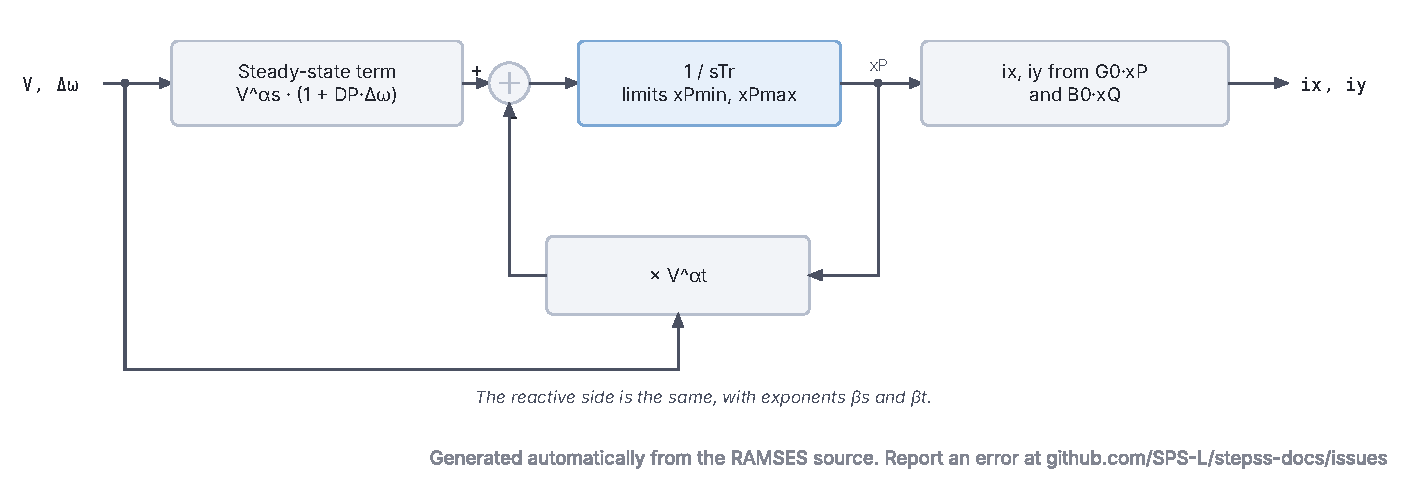
\includegraphics[width=0.98\linewidth]{figures/inj-restld-light}
\caption{Restorative load block diagram.}
\end{figure}

\subsection{Scientific Description}\label{model-inj-loads:scientific-description-2}

The recovery variable \(x_P\) for active power satisfies:

\[\dot{x}_P = \frac{1}{T_r}\left[V^{\alpha_s}\left(1 + D_P\,\Delta\omega\right) - x_P\, V^{\alpha_t}\right]\]

with analogous equation for \(x_Q\). Here \(\alpha_s\) and \(\alpha_t\) are the steady-state and transient voltage exponents respectively. Limiters \([x_{P,\min},\, x_{P,\max}]\) are applied. The injected currents are expressed as:

\[i_y = -B_0\left(1 + D_Q\,\Delta\omega\right) x_Q\, v_x + G_0\left(1 + D_P\,\Delta\omega\right) x_P\, v_y\]

\[i_x = \phantom{-}B_0\left(1 + D_Q\,\Delta\omega\right) x_Q\, v_y + G_0\left(1 + D_P\,\Delta\omega\right) x_P\, v_x\]

where the ratio \(V/V_0\) governs the voltage dependence through \texttt{vrat}.

\subsection{Parameters}\label{model-inj-loads:parameters-2}

\begin{small}\begin{longtable}[]{@{}llll@{}}
\toprule\noalign{}
\# & Name & Description & Unit \\
\midrule\noalign{}
\endhead
\bottomrule\noalign{}
\endlastfoot
1 & \texttt{DP} & Frequency sensitivity of active power & pu/pu \\
2 & \texttt{alphat} & Transient active power voltage exponent & \\
3 & \texttt{alphas} & Steady-state active power voltage exponent & \\
4 & \texttt{xP\_min} & Minimum limit for \(x_P\) & \\
5 & \texttt{xP\_max} & Maximum limit for \(x_P\) & \\
6 & \texttt{DQ} & Frequency sensitivity of reactive power & pu/pu \\
7 & \texttt{betat} & Transient reactive power voltage exponent & \\
8 & \texttt{betas} & Steady-state reactive power voltage exponent & \\
9 & \texttt{xQ\_min} & Minimum limit for \(x_Q\) & \\
10 & \texttt{xQ\_max} & Maximum limit for \(x_Q\) & \\
11 & \texttt{Tr} & Load recovery time constant & s \\
\end{longtable}\end{small}

\subsection{State Variables}\label{model-inj-loads:state-variables-2}

\begin{small}\begin{longtable}[]{@{}ll@{}}
\toprule\noalign{}
Variable & Description \\
\midrule\noalign{}
\endhead
\bottomrule\noalign{}
\endlastfoot
\texttt{iy} & \(y\)-component of injected current \\
\texttt{ix} & \(x\)-component of injected current \\
\texttt{xp} & Active power recovery variable \\
\texttt{xq} & Reactive power recovery variable \\
\end{longtable}\end{small}

\textbf{Observables:} \texttt{P}, \texttt{Q}, \texttt{xp}, \texttt{xq}

\subsection{Usage Example}\label{model-inj-loads:usage-example-2}

\begin{Verbatim}
INJEC  RESTLD  RESTLD1  BUS2
      # FP FQ P Q: share of the power-flow injection (FP, FQ) or initial power (P in MW, Q in Mvar)
      1.  1.  0.  0.
      # DP: Frequency sensitivity of active power (pu/pu)
      1.5
      # alphat: Active power exponent multiplying xP in the recovery equation
      2.0
      # alphas: Active power steady-state exponent in the recovery equation
      0.0
      # xP_min: Lower limit of active power recovery state xP
      0.0
      # xP_max: Upper limit of active power recovery state xP
      2.0
      # DQ: Frequency sensitivity of reactive power (pu/pu)
      1.2
      # betat: Reactive power exponent multiplying xQ in the recovery equation
      2.0
      # betas: Reactive power steady-state exponent in the recovery equation
      0.0
      # xQ_min: Lower limit of reactive power recovery state xQ
      0.0
      # xQ_max: Upper limit of reactive power recovery state xQ
      2.0
      # Tr: Load recovery time constant (s)
      60.0
;
\end{Verbatim}

\begin{center}\rule{0.5\linewidth}{0.5pt}\end{center}

\section{\texorpdfstring{PQ (\texttt{inj\_PQ}): Constant PQ Load}{PQ (inj\_PQ): Constant PQ Load}}\label{model-inj-loads:pq-inj_pq-constant-pq-load}

\subsection{Description}\label{model-inj-loads:description-3}

The simplest injector model: maintains constant active and reactive power consumption regardless of bus voltage or frequency. The power is fixed at its initial operating-point value. A small first-order filter (time constant \texttt{Tout}) drives the injected currents smoothly to their target values, preventing algebraic loops.

\begin{figure}[htbp]
\centering
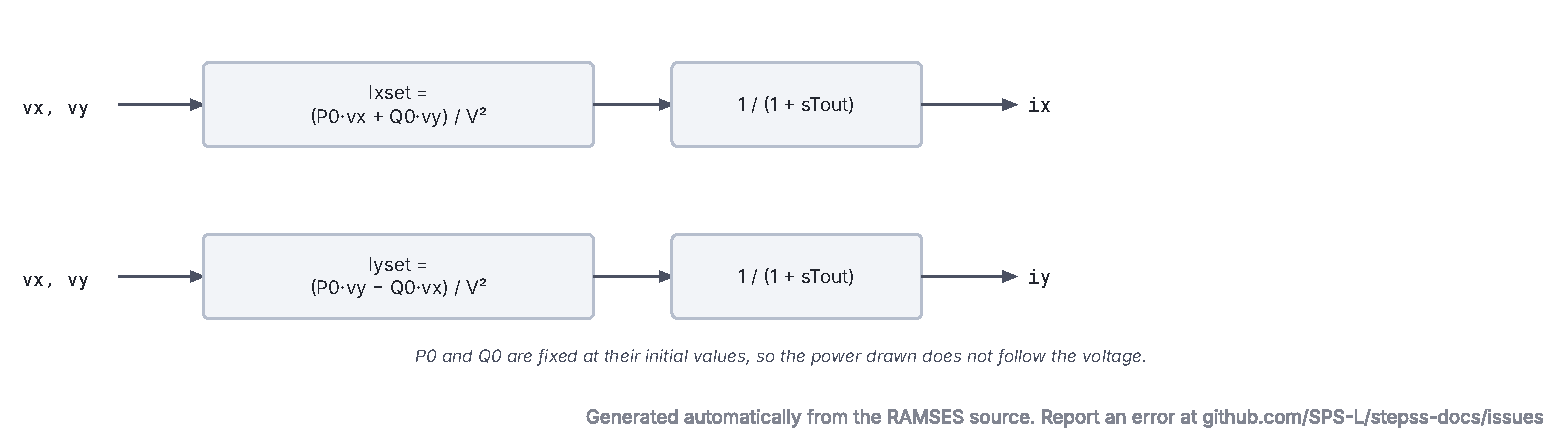
\includegraphics[width=0.98\linewidth]{figures/inj-pq-light}
\caption{Constant PQ load block diagram.}
\end{figure}

\subsection{Scientific Description}\label{model-inj-loads:scientific-description-3}

The current references are set to deliver the initial powers \(P_0\) and \(Q_0\) at the measured voltage \(V\):

\[I_{x,\mathrm{set}} = \frac{P_0 v_x + Q_0 v_y}{V^2}, \qquad I_{y,\mathrm{set}} = \frac{P_0 v_y - Q_0 v_x}{V^2}\]

These references pass through a first-order filter with time constant \(T_{\mathrm{out}}\) to produce the actual injected currents:

\[T_{\mathrm{out}}\,\dot{i}_x + i_x = I_{x,\mathrm{set}}, \qquad T_{\mathrm{out}}\,\dot{i}_y + i_y = I_{y,\mathrm{set}}\]

\subsection{Parameters}\label{model-inj-loads:parameters-3}

\begin{small}\begin{longtable}[]{@{}llll@{}}
\toprule\noalign{}
\# & Name & Description & Unit \\
\midrule\noalign{}
\endhead
\bottomrule\noalign{}
\endlastfoot
1 & \texttt{Tout} & Output filter time constant (recommended: 0.01 s) & s \\
\end{longtable}\end{small}

Initial conditions \(P_0\), \(Q_0\), \(V_0\) are computed automatically at initialization.

\subsection{State Variables}\label{model-inj-loads:state-variables-3}

\begin{small}\begin{longtable}[]{@{}ll@{}}
\toprule\noalign{}
Variable & Description \\
\midrule\noalign{}
\endhead
\bottomrule\noalign{}
\endlastfoot
\texttt{ix} & Injected \(x\)-current \\
\texttt{iy} & Injected \(y\)-current \\
\texttt{Ixset} & Current reference \(x\) \\
\texttt{Iyset} & Current reference \(y\) \\
\texttt{P} & Observed active power \\
\texttt{Q} & Observed reactive power \\
\texttt{V} & Bus voltage magnitude \\
\end{longtable}\end{small}

\textbf{Observables:} \texttt{P}, \texttt{Q}

\subsection{Usage Example}\label{model-inj-loads:usage-example-3}

\begin{Verbatim}
INJEC  inj_PQ  LOAD_PQ  BUS3
      # FP FQ P Q: share of the power-flow injection (FP, FQ) or initial power (P in MW, Q in Mvar)
      1.  1.  0.  0.
      # Tout: Output filter time constant (recommended: 0.01 s) (s)
      0.01
;
\end{Verbatim}

\begin{center}\rule{0.5\linewidth}{0.5pt}\end{center}

\section{\texorpdfstring{THEVEQ (\texttt{inj\_theveq}): Th\'evenin Equivalent}{THEVEQ (inj\_theveq): Th\'evenin Equivalent}}\label{model-inj-loads:theveq-inj_theveq-thuxe9venin-equivalent}

\subsection{Description}\label{model-inj-loads:description-4}

Models an external network or generator cluster as a Th\'evenin equivalent: an ideal voltage source \(\bar{E}_{\mathrm{th}}\) behind a pure reactance \(X_{\mathrm{th}}\). The model computes the internal voltage magnitude and phase angle at initialization from the initial bus conditions and holds them constant during the simulation. It is useful for representing neighbouring system equivalents or simplified machine representations.

\begin{figure}[htbp]
\centering
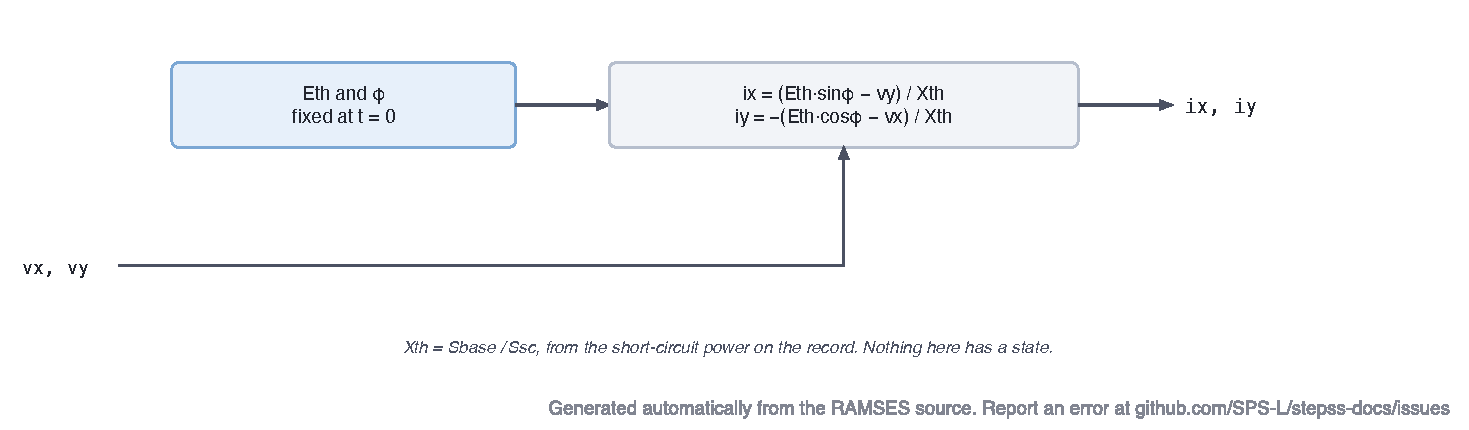
\includegraphics[width=0.98\linewidth]{figures/inj-theveq-light}
\caption{Thevenin equivalent block diagram.}
\end{figure}

\subsection{Scientific Description}\label{model-inj-loads:scientific-description-4}

The Th\'evenin reactance is obtained from the specified short-circuit power \(S_{\mathrm{sc}}\) (MVA):

\[X_{\mathrm{th}} = \frac{S_{\mathrm{base}}}{S_{\mathrm{sc}}}\]

The internal voltage phasor is computed at \(t=0\):

\[E_{\mathrm{th},x} = v_x - X_{\mathrm{th}}\, i_y, \qquad E_{\mathrm{th},y} = v_y + X_{\mathrm{th}}\, i_x\]

\[E_{\mathrm{th}} = \sqrt{E_{\mathrm{th},x}^2 + E_{\mathrm{th},y}^2}, \qquad \phi = \arctan\!\left(\frac{E_{\mathrm{th},y}}{E_{\mathrm{th},x}}\right)\]

During simulation the injected currents satisfy:

\[i_y = -\frac{E_{\mathrm{th}}\cos\phi - v_x}{X_{\mathrm{th}}}, \qquad i_x = \frac{E_{\mathrm{th}}\sin\phi - v_y}{X_{\mathrm{th}}}\]

\subsection{Parameters}\label{model-inj-loads:parameters-4}

\begin{small}\begin{longtable}[]{@{}
  >{\raggedright\arraybackslash}p{(\linewidth - 8\tabcolsep) * \real{0.0879}}
  >{\raggedright\arraybackslash}p{(\linewidth - 8\tabcolsep) * \real{0.1645}}
  >{\raggedright\arraybackslash}p{(\linewidth - 8\tabcolsep) * \real{0.5831}}
  >{\raggedright\arraybackslash}p{(\linewidth - 8\tabcolsep) * \real{0.1645}}
@{}}
\toprule\noalign{}
\begin{minipage}[b]{\linewidth}\raggedright
\#
\end{minipage} & \begin{minipage}[b]{\linewidth}\raggedright
Name
\end{minipage} & \begin{minipage}[b]{\linewidth}\raggedright
Description
\end{minipage} & \begin{minipage}[b]{\linewidth}\raggedright
Unit
\end{minipage} \\
\midrule\noalign{}
\endhead
\bottomrule\noalign{}
\endlastfoot
1 & \texttt{XTH} & Short-circuit power of the equivalent (converted to \(X_{\mathrm{th}}\) at initialization) & MVA \\
\end{longtable}\end{small}

Internal parameters \texttt{ETH} (Th\'evenin voltage magnitude, pu) and \texttt{phase} (internal angle, rad) are computed automatically.

\subsection{State Variables}\label{model-inj-loads:state-variables-4}

\begin{small}\begin{longtable}[]{@{}ll@{}}
\toprule\noalign{}
Variable & Description \\
\midrule\noalign{}
\endhead
\bottomrule\noalign{}
\endlastfoot
\texttt{iy} & Injected \(y\)-current \\
\texttt{ix} & Injected \(x\)-current \\
\end{longtable}\end{small}

\textbf{Observables:} \texttt{P}, \texttt{Q} (in MW and Mvar at system base)

\subsection{Usage Example}\label{model-inj-loads:usage-example-4}

\begin{Verbatim}
INJEC  THEVEQ  EQUIV1  SLACK_BUS
      # FP FQ P Q: share of the power-flow injection (FP, FQ) or initial power (P in MW, Q in Mvar)
      1.  1.  0.  0.
      # XTH: Short-circuit power of the equivalent (MVA)
      2000.0
;
\end{Verbatim}
